\chapter{Systembeskrivelse}
Det giver kapitel indeholder en gennemgang af den udviklede prototype, kaldet \textit{Konditioneringsapparatet}. Kapitlet har til formål at give læseren en forståelse af \textit{Konditioneringsapparatet} og for at sikre forståelsen af kommende kapitler. Det afsnit skal derfor ikke ses som værende en opsummering af projektets resultater, her henvises til kapitel \ref{title:resultater}.

\textit{Konditioneringsapparatet} er en prototype og et \textit{proof of concept} apparat der kan udføre konditioneringsbehandling og okklusionstræning. På figur \ref{fig:saelgertegning} ses en oversigt over systemet. For at kunne opfylde disse funktioner indeholder prototypen en række hardware og software dele. For at kunne lave en sikker og grundig afklemning 

\begin{figure}[H]
	\centering
	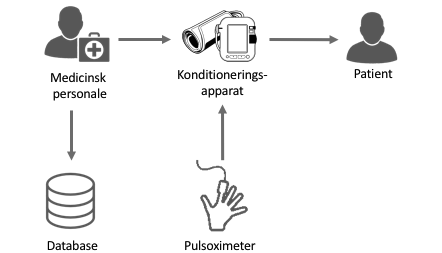
\includegraphics[width = 0.6\textwidth]{billeder/saelgertegning.png}
	\caption{Oversigt over \textit{Konditioneringsapparatet}} \label{fig:saelgertegning}
\end{figure}

\section{Brugergrænseflade}
\textit{Konditioneringsapparatets} brugergrænseflade består af 2 knapper og en skærm. Desuden findes en \textit{modeswitch} på prototypen, en \textit{modeswitch} er en knap med 3 stadier, som styre hvilke funktioner prototypen skal udføre. 